% rdwd package presentation
% Berry Boessenkool, Potsdam University, Germany
% berry-b@gmx.de

\documentclass[compress, xcolor=dvipsnames]{beamer}\usepackage[]{graphicx}\usepackage[]{color}
%% maxwidth is the original width if it is less than linewidth
%% otherwise use linewidth (to make sure the graphics do not exceed the margin)
\makeatletter
\def\maxwidth{ %
  \ifdim\Gin@nat@width>\linewidth
    \linewidth
  \else
    \Gin@nat@width
  \fi
}
\makeatother

\definecolor{fgcolor}{rgb}{0.345, 0.345, 0.345}
\newcommand{\hlnum}[1]{\textcolor[rgb]{0.686,0.059,0.569}{#1}}%
\newcommand{\hlstr}[1]{\textcolor[rgb]{0.192,0.494,0.8}{#1}}%
\newcommand{\hlcom}[1]{\textcolor[rgb]{0.678,0.584,0.686}{\textit{#1}}}%
\newcommand{\hlopt}[1]{\textcolor[rgb]{0,0,0}{#1}}%
\newcommand{\hlstd}[1]{\textcolor[rgb]{0.345,0.345,0.345}{#1}}%
\newcommand{\hlkwa}[1]{\textcolor[rgb]{0.161,0.373,0.58}{\textbf{#1}}}%
\newcommand{\hlkwb}[1]{\textcolor[rgb]{0.69,0.353,0.396}{#1}}%
\newcommand{\hlkwc}[1]{\textcolor[rgb]{0.333,0.667,0.333}{#1}}%
\newcommand{\hlkwd}[1]{\textcolor[rgb]{0.737,0.353,0.396}{\textbf{#1}}}%
\let\hlipl\hlkwb

\usepackage{framed}
\makeatletter
\newenvironment{kframe}{%
 \def\at@end@of@kframe{}%
 \ifinner\ifhmode%
  \def\at@end@of@kframe{\end{minipage}}%
  \begin{minipage}{\columnwidth}%
 \fi\fi%
 \def\FrameCommand##1{\hskip\@totalleftmargin \hskip-\fboxsep
 \colorbox{shadecolor}{##1}\hskip-\fboxsep
     % There is no \\@totalrightmargin, so:
     \hskip-\linewidth \hskip-\@totalleftmargin \hskip\columnwidth}%
 \MakeFramed {\advance\hsize-\width
   \@totalleftmargin\z@ \linewidth\hsize
   \@setminipage}}%
 {\par\unskip\endMakeFramed%
 \at@end@of@kframe}
\makeatother

\definecolor{shadecolor}{rgb}{.97, .97, .97}
\definecolor{messagecolor}{rgb}{0, 0, 0}
\definecolor{warningcolor}{rgb}{1, 0, 1}
\definecolor{errorcolor}{rgb}{1, 0, 0}
\newenvironment{knitrout}{}{} % an empty environment to be redefined in TeX

\usepackage{alltt}
\setbeamerfont{frametitle}{size=\normalsize}

\usepackage{hyperref, graphicx}
\usepackage[dvipsnames]{xcolor}
\renewcommand\appendixname{Appendix}
\usepackage[absolute,overlay]{textpos}
\hypersetup{colorlinks=true, linkcolor=blue, urlcolor=blue}
% \beamertemplatenavigationsymbolsempty
\setbeamertemplate{navigation symbols}[only frame symbol]
%\usetheme{Madrid}
\useoutertheme[subsection=false]{miniframes}
\beamersetleftmargin{0.5cm}
\beamersetrightmargin{0.5cm}
\let\Tiny=\tiny % avoid warning: Font shape `OT1/cmss/m/n' in size <4> not available. size <5> substituted on input line
\setbeamertemplate{footline}[frame number]

\newcommand{\bildlink}[1]{\flushleft{\tiny \href{#1}{\textcolor{gray}{#1}} \normalsize }}
\newcommand{\bildlinkt}[2]{\flushleft{\tiny \href{#1}{\textcolor{gray}{#2}} \normalsize }}



% ACTUAL SLIDES %%%%%%%%%%%%%%%%%%%%%%%%%%%%%%%%%%%%%%%%%%%%%%%%%%%%%%%%%%%%%%%%
\IfFileExists{upquote.sty}{\usepackage{upquote}}{}
\begin{document}
\centering


% ---------------------------

\section{Motivation}

% ---------------------------



% ---------------------------

\begin{frame}%[plain]
\vspace{1em}
\Large
\textbf{rdwd - an R package to select, download and read climate data from the German Weather Service}\\[2em]
\normalsize
Berry Boessenkool, \href{http://www.geo.uni-potsdam.de/geoecology.html}{uni-potsdam.de}, Feb 2017\\[1em]
\texttt{berry-b@gmx.de}\\[1em]
\href{https://github.com/brry/rdwd\#rdwd}{github.com/brry/rdwd}
\end{frame}

% ---------------------------

\begin{frame}{The German Weather Service (DWD) provides over 25'000 climate datasets}
\pause
\begin{itemize}%[<+->]
\item Too much for manual inspection
\item Somewhat difficult to search
\item File format inconsistent (e.g. column widths)
\end{itemize}
\pause
\flushleft{Screenshot of FTP server:}\\[0.5em]
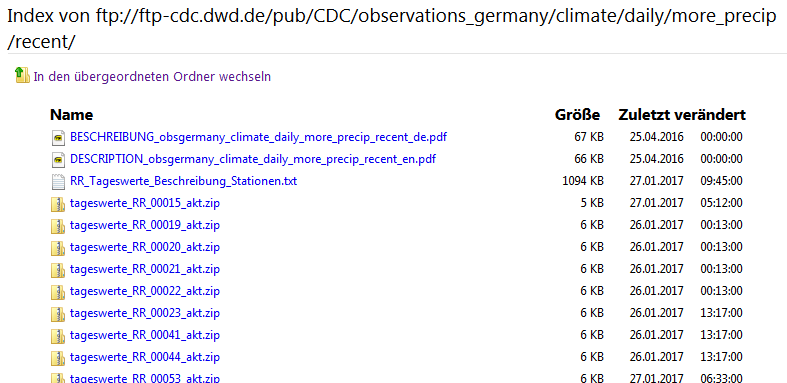
\includegraphics[width=0.9\textwidth]{dwd_ftp.PNG}\\
\end{frame}

% ---------------------------

\begin{frame}{R saves the day}
R package \texttt{rdwd} ~~$->$~~ easy usage of the datasets
\end{frame}

% ---------------------------

\begin{frame}{Overview}
\begin{itemize}%[<+->]
\item Motivation
\item Usage
\item Applications
\item Community
\end{itemize}
\end{frame}

% ---------------------------

\section{Usage}
\begin{frame}
\textbf{Usage}\\[1em]
- \hyperlink{ul}{get URL}\\
- \hyperlink{ud}{download}\\
- \hyperlink{ur}{read}\\
- \hyperlink{up}{plot}\\
- \hyperlink{um}{map}
\end{frame}

% ---------------------------

\begin{frame}[fragile]{U1/5: Get dataset URL with \texttt{selectDWD}}
\label{ul}
\pause
\begin{knitrout}
\definecolor{shadecolor}{rgb}{0.969, 0.969, 0.969}\color{fgcolor}\begin{kframe}
\begin{alltt}
\hlkwd{library}\hlstd{(}\hlstr{"rdwd"}\hlstd{)}
\end{alltt}
\end{kframe}
\end{knitrout}
\pause
\begin{knitrout}
\definecolor{shadecolor}{rgb}{0.969, 0.969, 0.969}\color{fgcolor}\begin{kframe}
\begin{alltt}
\hlstd{link} \hlkwb{<-} \hlkwd{selectDWD}\hlstd{(}\hlstr{"Potsdam"}\hlstd{,} \hlkwc{res}\hlstd{=}\hlstr{"daily"}\hlstd{,}
                  \hlkwc{var}\hlstd{=}\hlstr{"kl"}\hlstd{,} \hlkwc{per}\hlstd{=}\hlstr{"recent"}\hlstd{)}
\end{alltt}
\end{kframe}
\end{knitrout}
\pause
\begin{knitrout}
\definecolor{shadecolor}{rgb}{0.969, 0.969, 0.969}\color{fgcolor}\begin{kframe}
\begin{verbatim}
## ftp://ftp-cdc.dwd.de/pub/CDC/observations_germany/
## /climate/daily/kl/recent/tageswerte_KL_03987_akt.zip
\end{verbatim}
\end{kframe}
\end{knitrout}
\end{frame}

% ---------------------------

\begin{flushleft}

\begin{frame}[fragile]{U2/5: Download dataset with \texttt{dataDWD}}
\label{ud}
\pause
\begin{knitrout}
\definecolor{shadecolor}{rgb}{0.969, 0.969, 0.969}\color{fgcolor}\begin{kframe}
\begin{alltt}
\hlstd{file} \hlkwb{<-} \hlkwd{dataDWD}\hlstd{(link,} \hlkwc{read}\hlstd{=}\hlnum{FALSE}\hlstd{)}
\end{alltt}
\end{kframe}
\end{knitrout}
\begin{knitrout}\tiny
\definecolor{shadecolor}{rgb}{0.969, 0.969, 0.969}\color{fgcolor}\begin{kframe}


{\ttfamily\noindent\itshape\color{messagecolor}{\#\#\ \ dataDWD -> dirDWD: creating directory 'C:/Users/boessenkool/Dropbox/Public/rdwd/presentation/DWDdata'}}

{\ttfamily\noindent\itshape\color{messagecolor}{\#\#\ \ dataDWD -> fileDWD: creating 1 file: 'daily\_kl\_recent\_tageswerte\_KL\_03987\_akt.zip'}}\end{kframe}
\end{knitrout}
\pause
\begin{knitrout}
\definecolor{shadecolor}{rgb}{0.969, 0.969, 0.969}\color{fgcolor}\begin{kframe}
\begin{alltt}
\hlstd{file}
\end{alltt}
\begin{verbatim}
## [1] "daily_kl_recent_tageswerte_KL_03987_akt.zip"
\end{verbatim}
\end{kframe}
\end{knitrout}
\end{frame}
\end{flushleft}


% ---------------------------

\begin{frame}[fragile]{U3/5: Unzip file and read + convert data with \texttt{readDWD}}
\label{ur}
\pause
\begin{knitrout}
\definecolor{shadecolor}{rgb}{0.969, 0.969, 0.969}\color{fgcolor}\begin{kframe}
\begin{alltt}
\hlstd{clim} \hlkwb{<-} \hlkwd{readDWD}\hlstd{(file)}
\end{alltt}
\end{kframe}
\end{knitrout}
\pause
\begin{knitrout}\tiny
\definecolor{shadecolor}{rgb}{0.969, 0.969, 0.969}\color{fgcolor}\begin{kframe}
\begin{alltt}
\hlkwd{str}\hlstd{(clim)}
\end{alltt}
\begin{verbatim}
## 'data.frame':	550 obs. of  18 variables:
##  $ STATIONS_ID             : int  3987 3987 3987 3987 3987 3987 3987 3987 3987 3987 ...
##  $ MESS_DATUM              : POSIXct, format: "2015-08-02" "2015-08-03" ...
##  $ QUALITAETS_NIVEAU       : int  3 3 3 3 3 3 3 3 3 3 ...
##  $ LUFTTEMPERATUR          : num  22.4 23.8 25.8 20.6 25.2 27.8 24.5 22.5 25.3 25.8 ...
##  $ DAMPFDRUCK              : num  11.7 13.3 15.7 15.4 15.8 17.4 18.6 15.3 17.7 19.1 ...
##  $ BEDECKUNGSGRAD          : num  4.5 2 2.9 4.9 3.6 3.4 4.4 2.3 3.3 4 ...
##  $ LUFTDRUCK_STATIONSHOEHE : num  1007 1006 1002 1007 1004 ...
##  $ REL_FEUCHTE             : num  46.8 49.4 52.4 66.2 54.1 ...
##  $ WINDGESCHWINDIGKEIT     : num  3 3 5 3.4 3.4 4 4.3 3.5 3.8 3.8 ...
##  $ LUFTTEMPERATUR_MAXIMUM  : num  30 32.3 35.3 26.3 34.6 37.6 33.3 29.5 33.5 33.1 ...
##  $ LUFTTEMPERATUR_MINIMUM  : num  15.1 14 18.4 16.4 16.1 21.2 19.2 16.6 17.1 19.4 ...
##  $ LUFTTEMP_AM_ERDB_MINIMUM: num  11.6 11.7 16.1 14.9 13.5 18.1 17.8 15.5 16.1 18.7 ...
##  $ WINDSPITZE_MAXIMUM      : num  8.1 9.2 17.3 9.1 9.6 9.1 12.5 8.2 8.4 11.7 ...
##  $ NIEDERSCHLAGSHOEHE      : num  0 0 4.1 0 0 0 0.1 0 0 0 ...
##  $ NIEDERSCHLAGSHOEHE_IND  : int  0 0 6 0 0 0 6 0 0 0 ...
##  $ SONNENSCHEINDAUER       : num  13.4 14.4 11.6 10.7 13.3 ...
##  $ SCHNEEHOEHE             : int  0 0 0 0 0 0 0 0 0 0 ...
##  $ eor                     : Factor w/ 1 level "eor": 1 1 1 1 1 1 1 1 1 1 ...
\end{verbatim}
\end{kframe}
\end{knitrout}
\end{frame}

% ---------------------------

\begin{frame}[fragile]{U4/5: Data can be plotted with regular R code}
\label{up}
\pause
\begin{knitrout}
\definecolor{shadecolor}{rgb}{0.969, 0.969, 0.969}\color{fgcolor}\begin{kframe}
\begin{alltt}
\hlkwd{plot}\hlstd{(clim[,}\hlkwd{c}\hlstd{(}\hlnum{2}\hlstd{,}\hlnum{4}\hlstd{)],} \hlkwc{type}\hlstd{=}\hlstr{"l"}\hlstd{,} \hlkwc{xaxt}\hlstd{=}\hlstr{"n"}\hlstd{,} \hlkwc{las}\hlstd{=}\hlnum{1}\hlstd{)}
\hlstd{berryFunctions}\hlopt{::}\hlkwd{monthAxis}\hlstd{(}\hlkwc{ym}\hlstd{=}\hlnum{TRUE}\hlstd{)   ;}   \hlkwd{abline}\hlstd{(}\hlkwc{h}\hlstd{=}\hlnum{0}\hlstd{)}
\end{alltt}
\end{kframe}
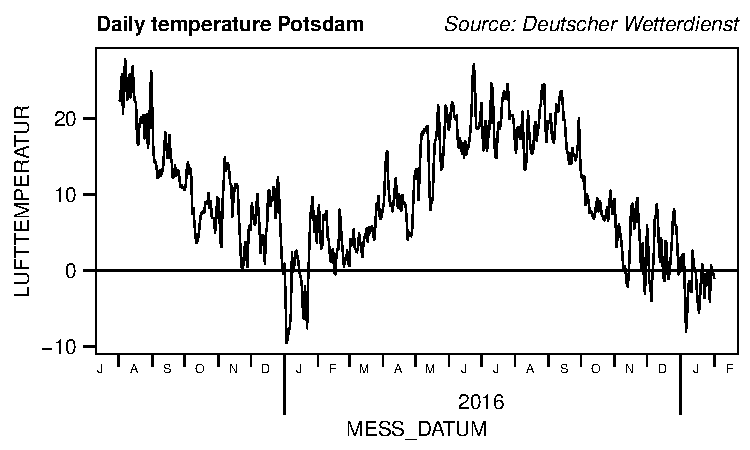
\includegraphics[width=0.9\textwidth]{figure/tempplot-1} 

\end{knitrout}
\end{frame}

% ---------------------------

% \begin{frame}{\texttt{rdwd}: assessing the power of DWD data}
% 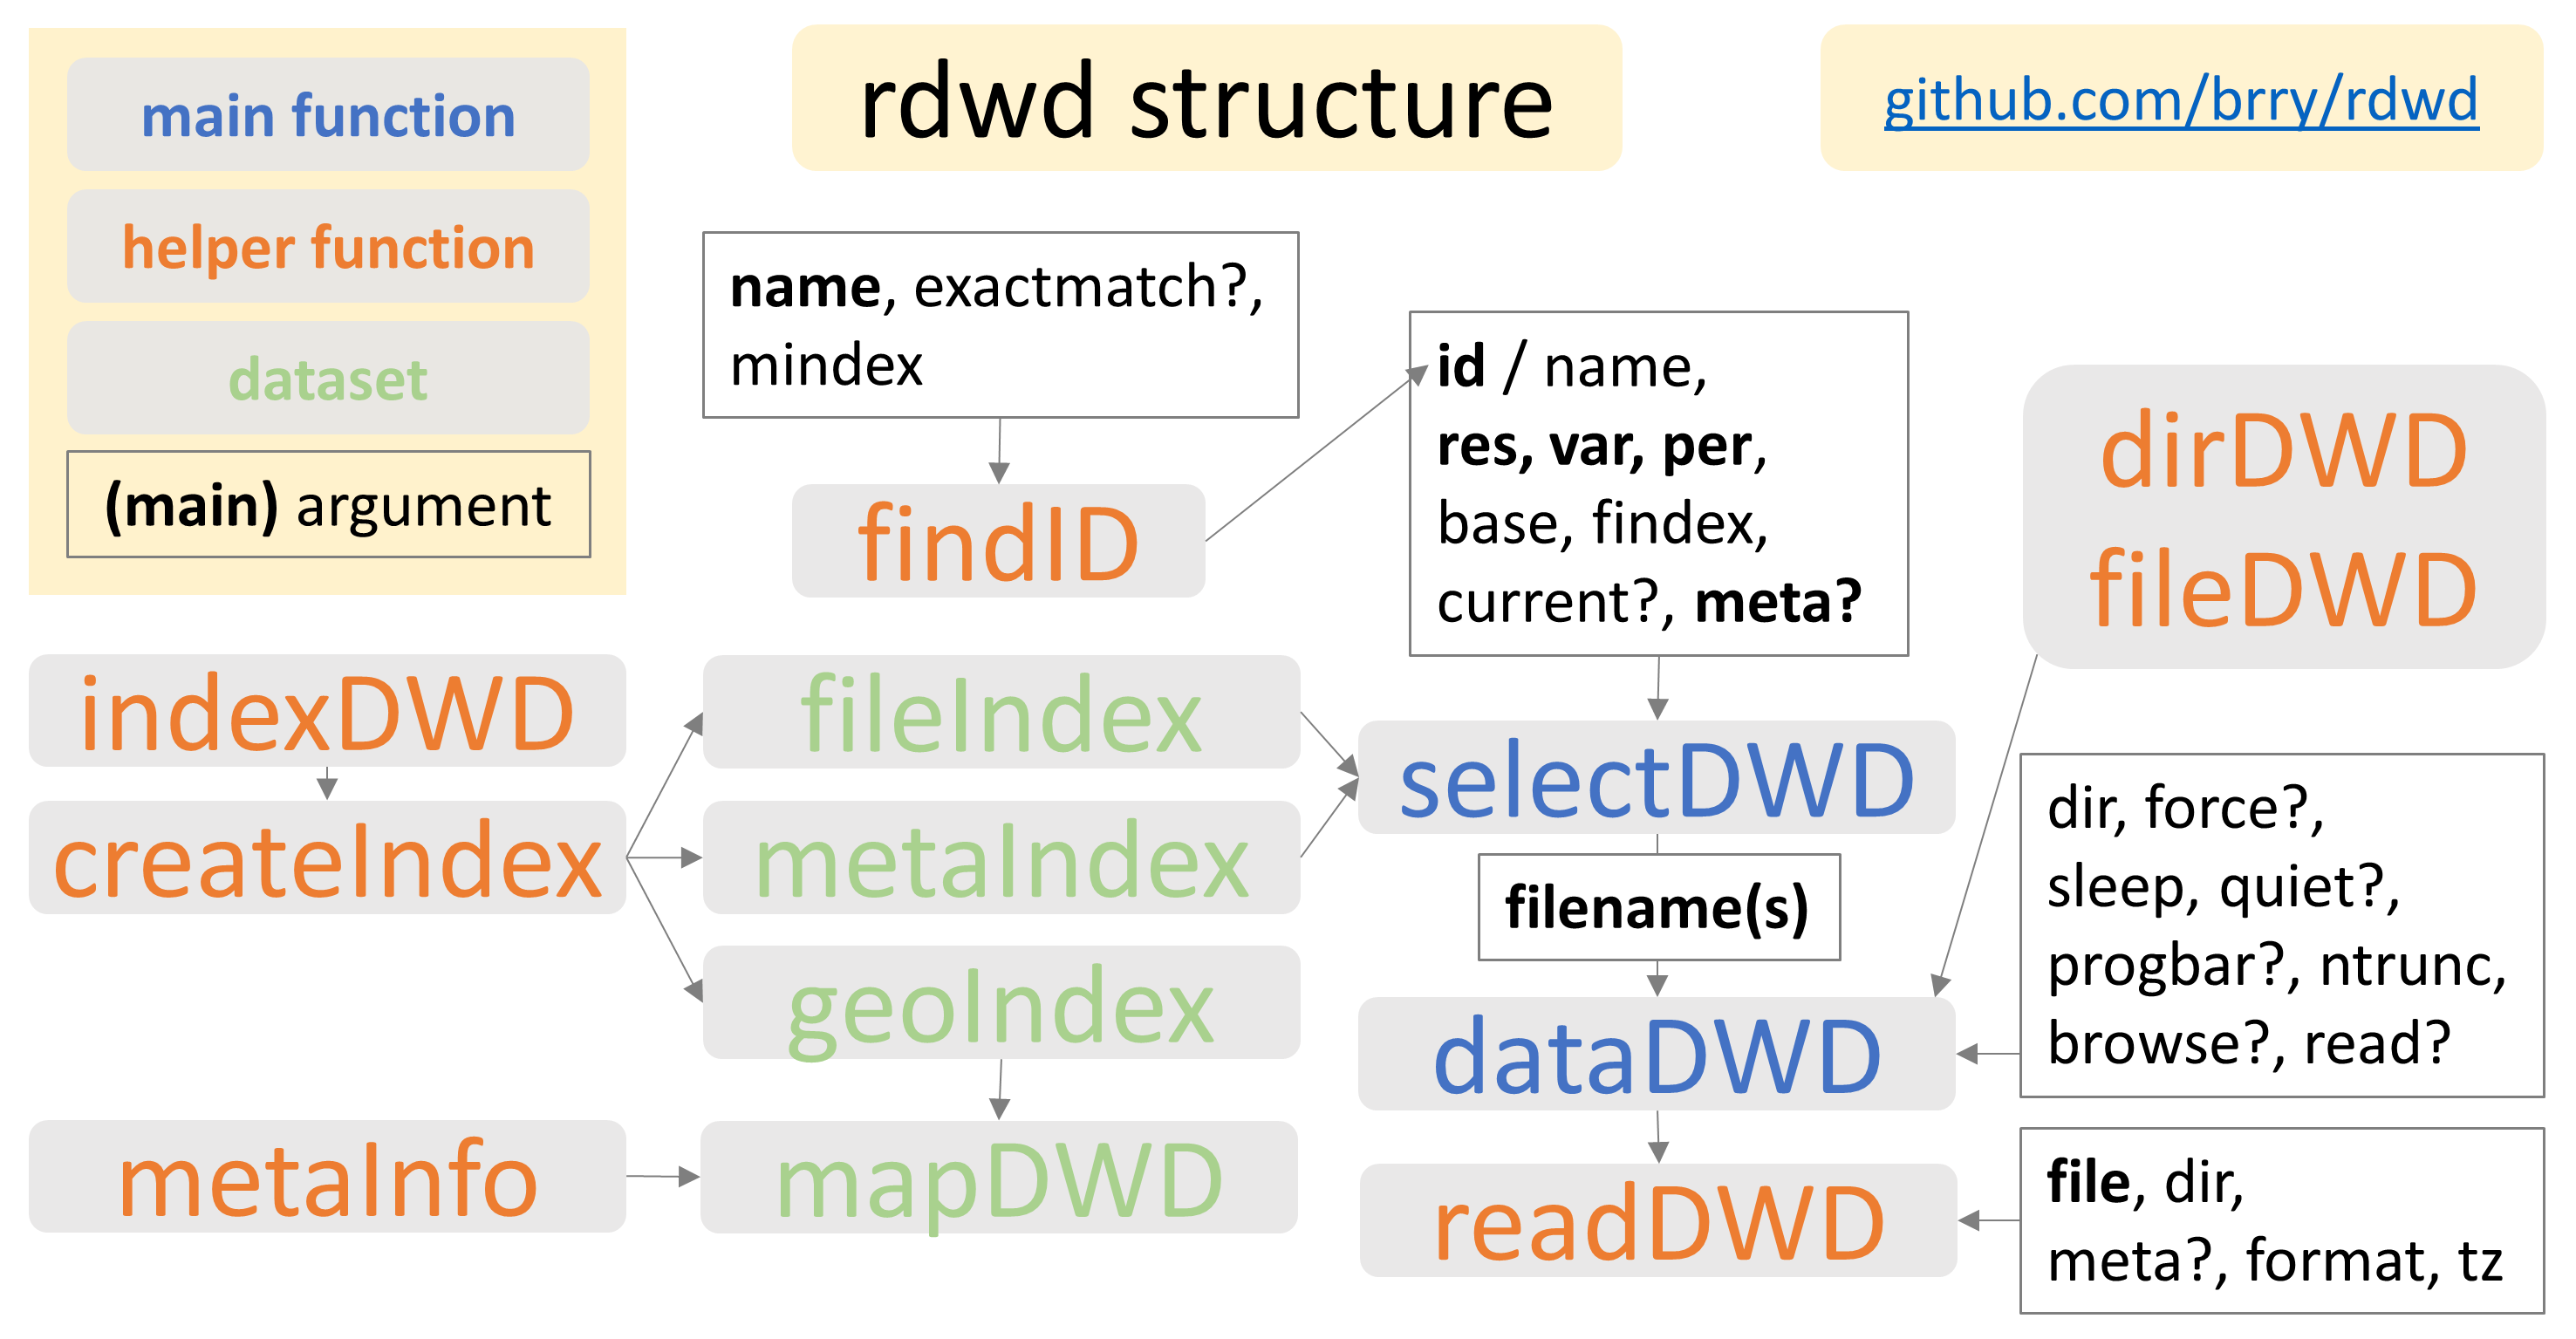
\includegraphics[width=0.99\textwidth]{../vignettes/PackageSchematic.png}
% \end{frame}

% ---------------------------

\begin{frame}[fragile]{U5/5: Interactive map (\href{../inst/doc/mapDWD.html}{local})}
\label{um}
\begin{knitrout}
\definecolor{shadecolor}{rgb}{0.969, 0.969, 0.969}\color{fgcolor}\begin{kframe}
\begin{alltt}
\hlkwd{vignette}\hlstd{(}\hlstr{"mapDWD"}\hlstd{,} \hlkwc{package}\hlstd{=}\hlstr{"rdwd"}\hlstd{)}
\end{alltt}
\end{kframe}
\end{knitrout}
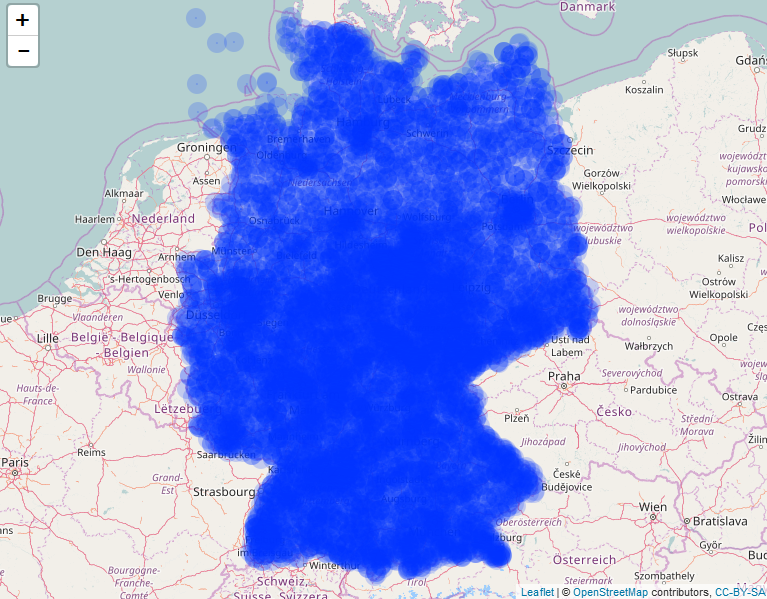
\includegraphics[width=0.7\textwidth]{map1.png}
\end{frame}

% ---------------------------

\begin{frame}[fragile]{U5/5: Interactive map (\href{https://cran.r-project.org/web/packages/rdwd/vignettes/mapDWD.html}{CRAN})}
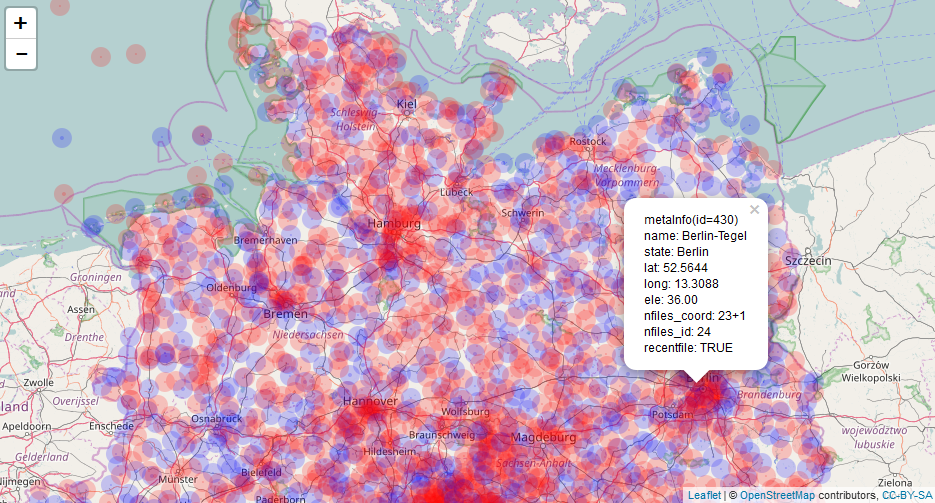
\includegraphics[width=0.99\textwidth]{map2.png}
\end{frame}

% ---------------------------
\section{Applications}
\begin{frame}
\textbf{Applications}\\[1em]
- \hyperlink{ac}{climate graph}\\
- \hyperlink{ae}{event analysis}\\
- \hyperlink{ar}{rainfall extremes}\\
\end{frame}

% ---------------------------

\begin{frame}[fragile]{A1/3: Long term climate graph (Potsdam 1893:2015)}
\label{ac}
\begin{knitrout}
\definecolor{shadecolor}{rgb}{0.969, 0.969, 0.969}\color{fgcolor}\begin{kframe}
\begin{alltt}
\hlstd{clim} \hlkwb{<-} \hlkwd{dataDWD}\hlstd{(}\hlkwd{selectDWD}\hlstd{(}\hlstr{"Potsdam"}\hlstd{,} \hlkwc{res}\hlstd{=}\hlstr{"monthly"}\hlstd{,}
                          \hlkwc{var}\hlstd{=}\hlstr{"kl"}\hlstd{,} \hlkwc{per}\hlstd{=}\hlstr{"h"}\hlstd{))}
\hlstd{clim}\hlopt{$}\hlstd{month} \hlkwb{<-} \hlkwd{substr}\hlstd{(clim}\hlopt{$}\hlstd{MESS_DATUM_BEGINN,}\hlnum{5}\hlstd{,}\hlnum{6}\hlstd{)}
\hlstd{temp} \hlkwb{<-} \hlkwd{tapply}\hlstd{(clim}\hlopt{$}\hlstd{LUFTTEMPERATUR, clim}\hlopt{$}\hlstd{month, mean)}
\hlstd{prec} \hlkwb{<-} \hlkwd{tapply}\hlstd{(clim}\hlopt{$}\hlstd{NIEDERSCHLAGSHOEHE, clim}\hlopt{$}\hlstd{month, mean)}
\hlstd{berryFunctions}\hlopt{::}\hlkwd{climateGraph}\hlstd{(temp, prec,} \hlkwc{main}\hlstd{=}\hlstr{""}\hlstd{)}
\end{alltt}
\end{kframe}
\end{knitrout}
\end{frame}

% ---------------------------

\begin{frame}[fragile]{A1/3: Long term climate graph (Potsdam 1893:2015)}
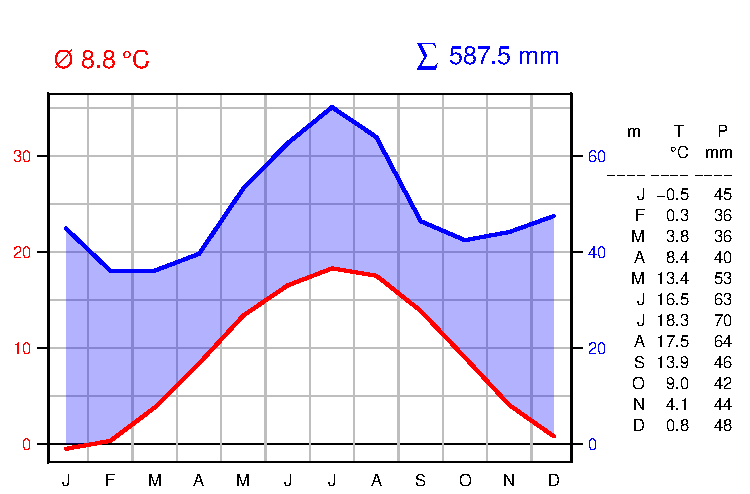
\includegraphics[width=0.99\textwidth]{figure/climgraph-1.pdf}
\end{frame}

% ---------------------------

\begin{frame}[fragile]{A2/3: Flashflood event rainfall analysis (\href{http://www.uni-potsdam.de/natriskchange/qualification-program/task-force-braunsbach-flash-flood-2016.html}{Taskforce report})}
\label{ae}
\pause
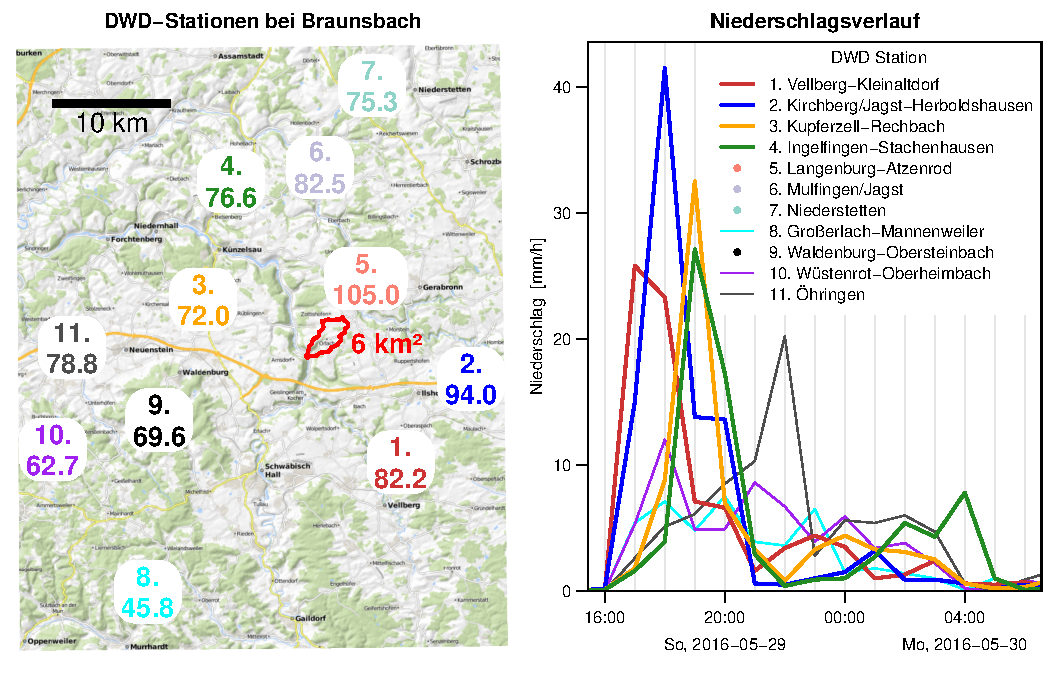
\includegraphics[width=0.99\textwidth]{Rainfall_map_events.pdf}
\end{frame}

% ---------------------------

\begin{frame}{A3/3: Extreme rainfall over temperature (\href{https://github.com/brry/prectemp}{github.com/brry/prectemp})}
\label{ar}
\only<1>{
\textblockcolour{white}
\begin{textblock*}{5.1cm}(6.5cm,1.4cm)
\vspace{7.0cm} ~
\end{textblock*}
\vspace{0.1em}
}
\only<1-2>{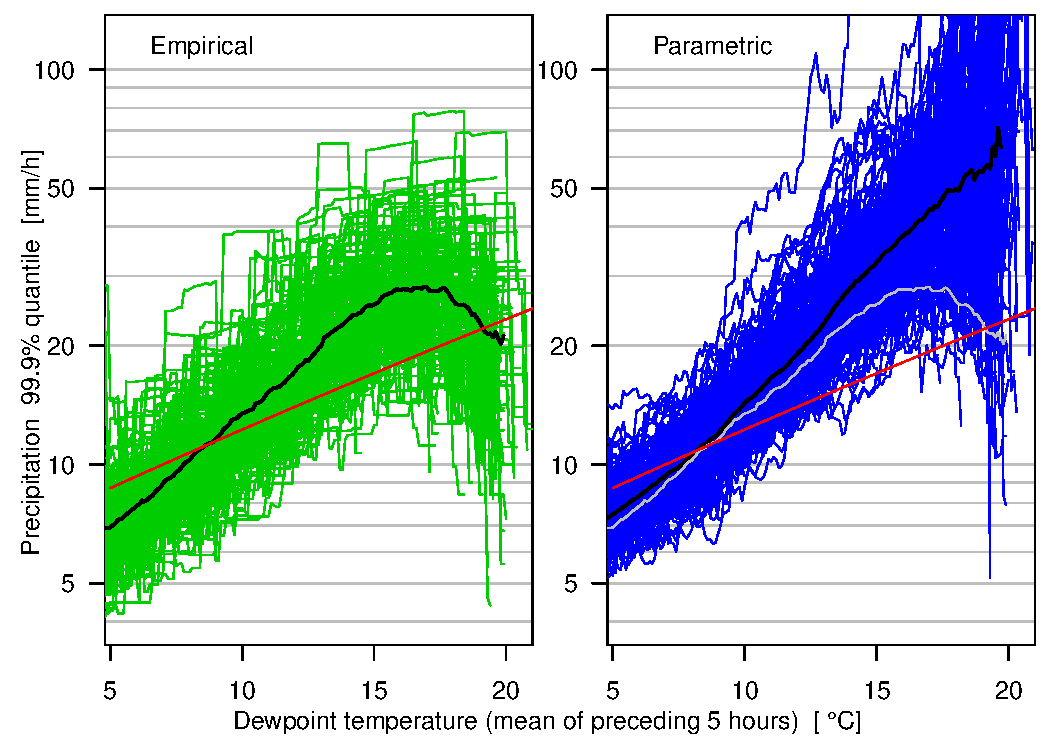
\includegraphics[width=0.9\textwidth]{fig2.pdf}}
\end{frame}

% ---------------------------

\section{Community}

% ---------------------------

\begin{frame}{The FOSS community role}
\pause
\begin{itemize}[<+->]
\item Stackoverflow for programming help
\item Lobbying DWD into publishing tax-paid data
\item Package distribution infrastructure (CRAN)
\item \texttt{leaflet} interactive map really easy to create
\end{itemize}
\end{frame}

% ---------------------------

\begin{frame}{Conclusion}
\pause
\begin{itemize}[<+->]
\item FOSS is awesome
\item DWD is awesome
\item Usage of the data is easy with \texttt{rdwd}
\end{itemize}
\end{frame}

% ---------------------------

\end{document}

